\documentclass[]{article}

\usepackage{amsmath}
\usepackage{makeidx}
\usepackage{lscape}
\usepackage{graphicx}
	 
%opening
\title{Report on panel model results}
\author{Vicente López Díaz}
\makeindex

\begin{document}

\maketitle


\begin{abstract}
These note is to relate several models that can use panel data.
\end{abstract}

The objective of these note is to give a broad overview of the possible models that can use panel data. There are several usual features to consider in a model with panel data, for example, changes on parameters for time or individual. Also, specification on error term is relevant for interpretation.

The note is based on Hsiao (2014). It goes from the theory in the text, to the application.

\section{Data plots}
Here is a summary of the data available for the analysis. 

Figure 1 presents the initial data points, these are used for the analysis.

I made a decision on which brands to include based on the number of observations on the period previous to the tax implementation, the tax started in january 2021, I made an exploratory analysis on the december 2020 data. This would ease the inclusion of brand explicitly in the analysis, brands with few observations, with difficulties to calculate most estimates could be analyzed after applying some criteria to make groups of brands out of the individual ones.


\begin{figure}
\begin{center}
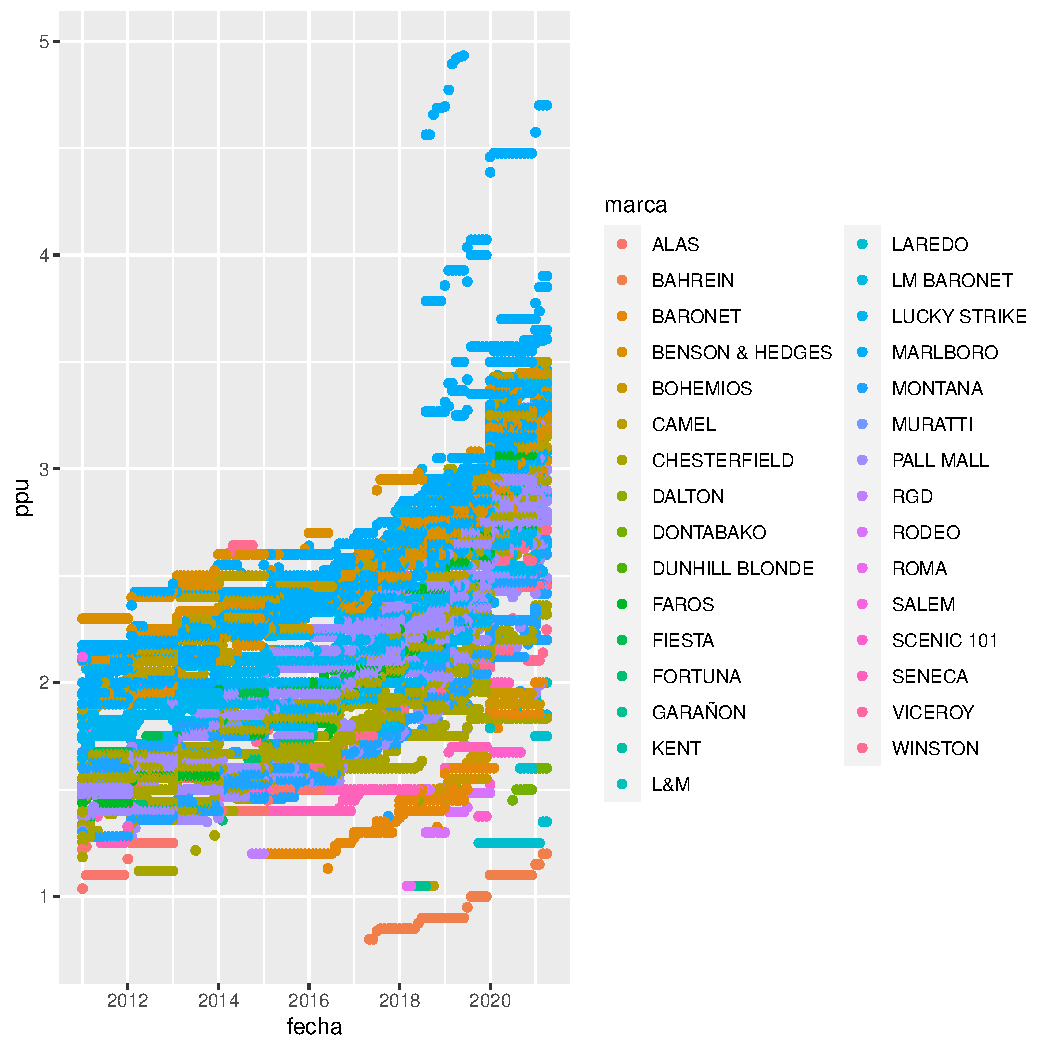
\includegraphics[width=\textwidth]{df_review_ppu_marcas.pdf} 
\end{center}
 \caption{All brands average price per unit}
\end{figure}

Figure 2 only considers the 7 most frequent brands. The graph provides some guidance on what to consider for the proposed descriptive model.  In particular, there is clear trend over time and there are price adjustments in january. 

\begin{figure}
\begin{center}
		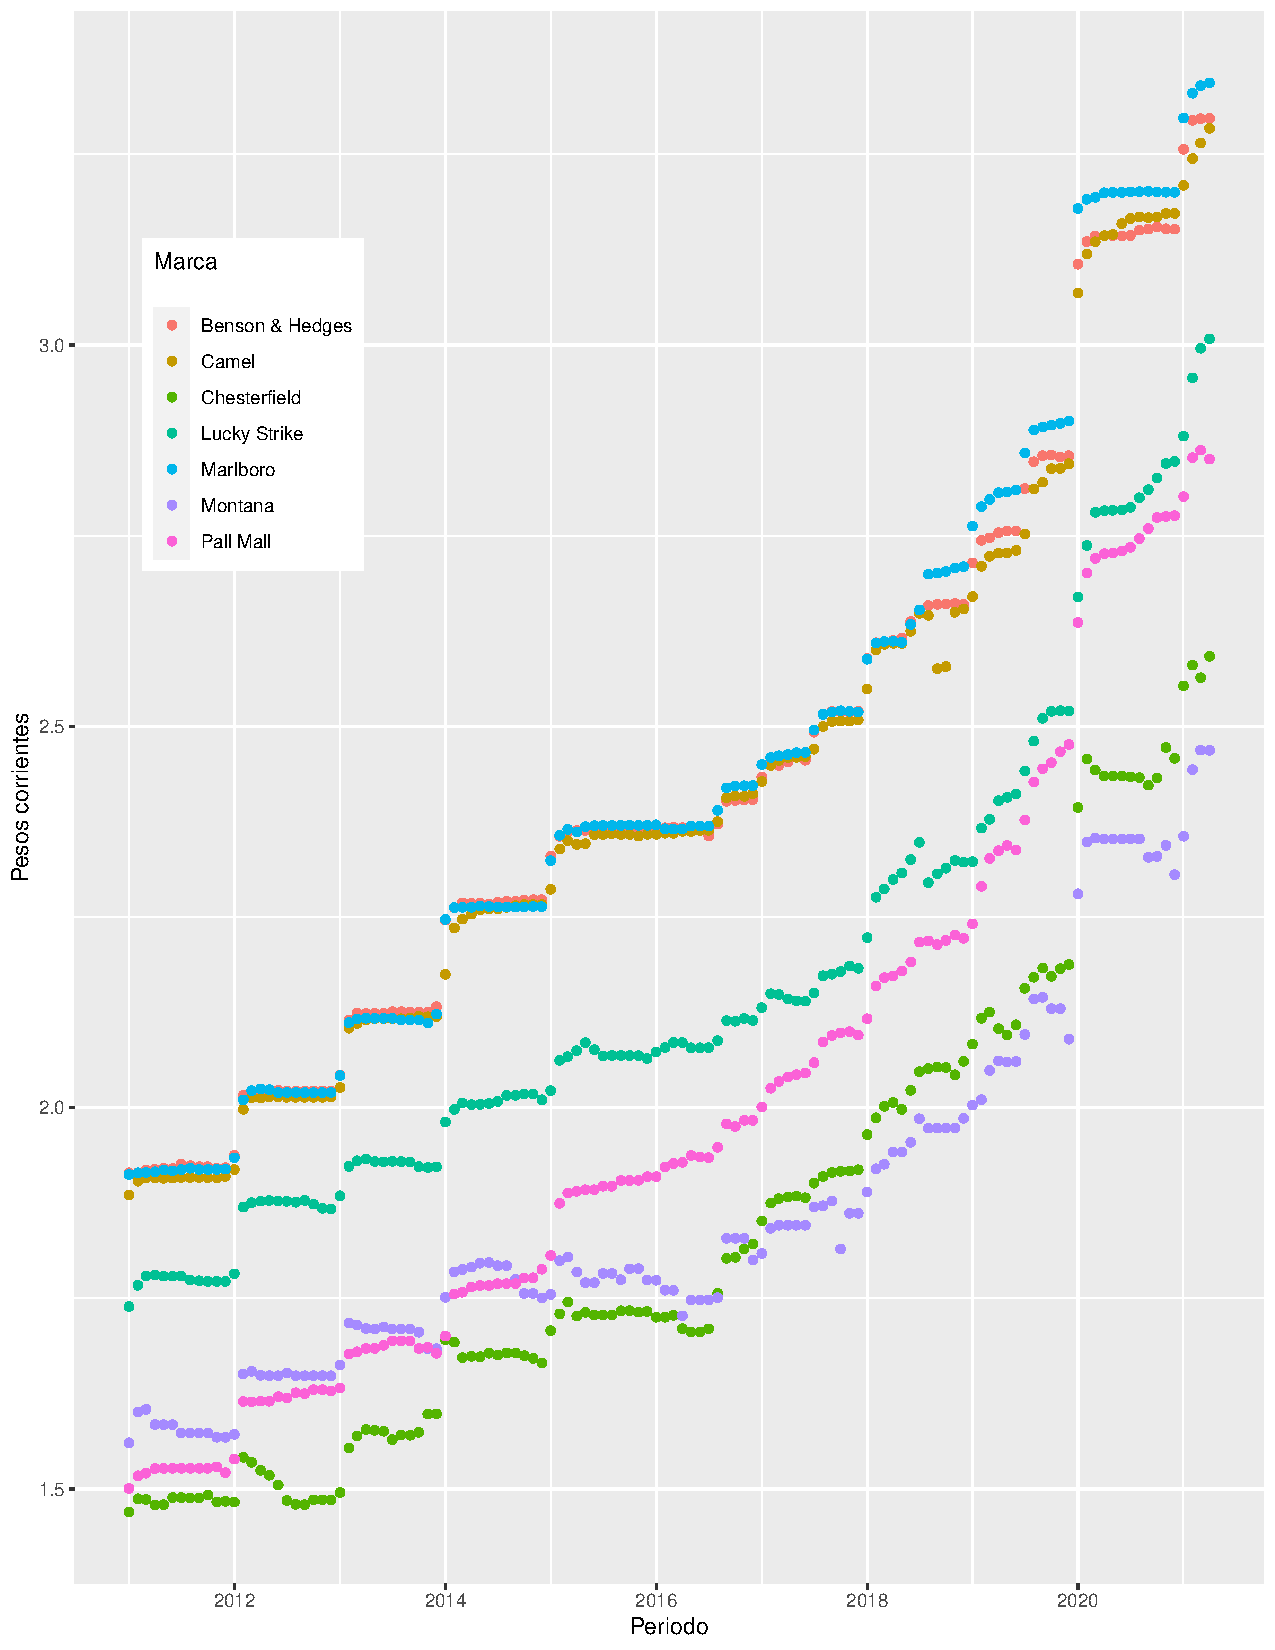
\includegraphics[width=\textwidth]{prin7_prom_ppu_marcas.pdf} 
\end{center}
 \caption{Seven brands average price per unit}
\end{figure}


Except for prices of other products, there are no other potential regressors to consider at the same level of the data.

\section{Dummies for each level: city, brand, time}
Estimations using areg, fixed effects are imposed. Using  this method there is one category with parameters "absorbed", which are not estimated as a result of the procedure.

Specification with indicators for city, brand and trend for time.
Same tax effect on all the brands.

\begin{equation*} 
y_{itm}  = \alpha_{i}^{*} + \gamma_{m}^{*} + \lambda*t + \beta_{0}^{'}jan + \beta_{1}^{'}tax2020 + \beta_{1}^{'}tax2021 + u_{itm}
;   \tag{2.1}
\end{equation*}
$c  = 1,\ldots,N;  t=1,\ldots,T; m=1,\ldots,M. $

Specification with indicators for city, brand and trend for time.
Effect interacted for each brand.

\begin{equation*} 
	y_{ctm}  = \alpha_{i}^{*} + \gamma_{m}^{*} + \lambda*t + \beta_{0}^{'}jan + \beta_{1m}^{'}tax2020 + \beta_{2m}^{'}tax2021 + u_{itm}
	;   \tag{2.2}
\end{equation*}
$c  = 1,\ldots,N;  t=1,\ldots,T; m=1,\ldots,M. $

Results with data for the 7 brands:

\begin{longtable}{lcccc} 
\caption{Fixed Effects for city and brand combination}\label{tab:1}\\	
	\hline
 & (1) & (2) & (3) & (4) \\
%\begin{tabular}{lcccc} \hline
%	& (1) & (2) & (3) & (4) \\
VARIABLES & ppu & ppu & ppu & ppu \\ \hline
 &  &  &  &  \\
jan20 & 0.209*** & 0.238*** & -0.017* & 0.012 \\
& (0.011) & (0.024) & (0.009) & (0.018) \\
jan21 & 0.242*** & 0.285*** & -0.011 & 0.032* \\
& (0.011) & (0.024) & (0.010) & (0.019) \\
jan & -0.024*** & -0.024*** & -0.069*** & -0.069*** \\
& (0.004) & (0.004) & (0.004) & (0.004) \\
jan20\#2.marca &  & -0.007 &  & -0.012 \\
 &  & (0.042) &  & (0.032) \\
jan20\#3.marca &  & -0.111** &  & -0.112*** \\
 &  & (0.043) &  & (0.033) \\
jan20\#4.marca &  & -0.147*** &  & -0.150*** \\
 &  & (0.039) &  & (0.030) \\
jan20\#5.marca &  & 0.052 &  & 0.051** \\
 &  & (0.032) &  & (0.024) \\
jan20\#6.marca &  & -0.239*** &  & -0.235*** \\
 &  & (0.062) &  & (0.048) \\
jan20\#7.marca &  & -0.028 &  & -0.024 \\
 &  & (0.034) &  & (0.026) \\
jan21\#2.marca &  & -0.035 &  & -0.040 \\
 &  & (0.040) &  & (0.031) \\
jan21\#3.marca &  & -0.116** &  & -0.118*** \\
 &  & (0.046) &  & (0.035) \\
jan21\#4.marca &  & -0.132*** &  & -0.134*** \\
 &  & (0.038) &  & (0.029) \\
jan21\#5.marca &  & 0.022 &  & 0.021 \\
 &  & (0.032) &  & (0.024) \\
jan21\#6.marca &  & -0.361*** &  & -0.357*** \\
 &  & (0.063) &  & (0.048) \\
jan21\#7.marca &  & -0.036 &  & -0.031 \\
 &  & (0.034) &  & (0.026) \\
2.marca & -0.012*** & -0.011*** & -0.006** & -0.006** \\
& (0.003) & (0.003) & (0.003) & (0.003) \\
3.marca & -0.595*** & -0.593*** & -0.592*** & -0.591*** \\
& (0.004) & (0.004) & (0.003) & (0.003) \\
4.marca & -0.270*** & -0.268*** & -0.268*** & -0.266*** \\
& (0.003) & (0.003) & (0.003) & (0.003) \\
5.marca & 0.011*** & 0.010*** & 0.011*** & 0.010*** \\
& (0.003) & (0.003) & (0.002) & (0.002) \\
6.marca & -0.524*** & -0.521*** & -0.527*** & -0.524*** \\
& (0.005) & (0.005) & (0.004) & (0.004) \\
7.marca & -0.435*** & -0.435*** & -0.441*** & -0.440*** \\
& (0.003) & (0.003) & (0.002) & (0.002) \\
ym & 0.009*** & 0.009*** &  &  \\
 & (0.000) & (0.000) &  &  \\
Constant & -3.925*** & -3.926*** & 1.991*** & 1.990*** \\
 & (0.018) & (0.018) & (0.004) & (0.004) \\
 &  &  &  &  \\
Observations & 24,010 & 24,010 & 24,010 & 24,010 \\
 R-squared & 0.897 & 0.897 & 0.940 & 0.940 \\ \hline
\multicolumn{5}{c}{ Standard errors in parentheses} \\
\multicolumn{5}{c}{ *** p$<$0.01, ** p$<$0.05, * p$<$0.1} \\
%\end{tabular}
\end{longtable}


The columns 1 and 3 consider the same effect for each brand, the columns 2 and 4 estimate a different effect for each brand. The columns 1 and 2 consider a trend, columns 3 and 4 use a combination of dummy variables for year and month.

MANUAL: REMOVE THE CATEGORIES ZERO IN m1-20.marca

\subsection{Comparisons by segment}

Results for brand type: 1 is premium, 2 is medium, 3 is low.

\begin{longtable}{lcccccc} 
	\caption{Fixed Effects by brand type}\label{tab:2}\\	
	\hline
%\begin{tabular}{lcccccc} \hline
 & (1) & (2) & (3) & (4) & (5) & (6) \\
VARIABLES & ppu & ppu & ppu & ppu & ppu & ppu \\ \hline
 &  &  &  &  &  &  \\
jan20 & 0.219*** & 0.198*** & 0.182*** & 0.119*** & 0.191*** & 0.225*** \\
& (0.012) & (0.019) & (0.021) & (0.033) & (0.034) & (0.040) \\
jan21 & 0.238*** & 0.235*** & 0.235*** & 0.188*** & 0.231*** & 0.310*** \\
& (0.012) & (0.019) & (0.021) & (0.033) & (0.036) & (0.042) \\
jan & -0.018*** & -0.018*** & -0.040*** & -0.040*** & -0.013 & -0.013 \\
& (0.004) & (0.004) & (0.007) & (0.007) & (0.009) & (0.009) \\
jan20\#2.marca &  & -0.009 &  &  &  &  \\
 &  & (0.032) &  &  &  &  \\
jan20\#5.marca &  & 0.051** &  &  &  &  \\
&  & (0.025) &  &  &  &  \\
jan20\#6.marca &  &  &  &  &  & -0.119* \\
&  &  &  &  &  & (0.072) \\
jan20\#7.marca &  &  &  & 0.102** &  &  \\
&  &  &  & (0.041) &  &  \\
jan21\#2.marca &  & -0.037 &  &  &  &  \\
 &  & (0.031) &  &  &  &  \\
jan21\#5.marca &  & 0.022 &  &  &  &  \\
 &  & (0.025) &  &  &  &  \\
jan21\#6.marca &  &  &  &  &  & -0.252*** \\
&  &  &  &  &  & (0.073) \\
jan21\#7.marca &  &  &  & 0.076* &  &  \\
&  &  &  & (0.040) &  &  \\
2.marca & -0.008*** & -0.007*** &  &  &  &  \\
& (0.003) & (0.003) &  &  &  &  \\
5.marca & 0.008*** & 0.007*** &  &  &  &  \\
& (0.002) & (0.002) &  &  &  &  \\
6.marca &  &  &  &  & 0.101*** & 0.102*** \\
&  &  &  &  & (0.007) & (0.007) \\
7.marca &  &  & -0.165*** & -0.166*** &  &  \\
&  &  & (0.004) & (0.004) &  &  \\
ym & 0.010*** & 0.010*** & 0.009*** & 0.009*** & 0.007*** & 0.007*** \\
 & (0.000) & (0.000) & (0.000) & (0.000) & (0.000) & (0.000) \\
Constant & -4.429*** & -4.429*** & -4.040*** & -4.041*** & -2.892*** & -2.895*** \\
 & (0.019) & (0.019) & (0.037) & (0.037) & (0.051) & (0.051) \\
 &  &  &  &  &  &  \\
Observations & 13,396 & 13,396 & 6,700 & 6,700 & 3,914 & 3,914 \\
 R-squared & 0.917 & 0.918 & 0.846 & 0.846 & 0.760 & 0.761 \\ \hline
\multicolumn{7}{c}{ Standard errors in parentheses} \\
\multicolumn{7}{c}{ *** p$<$0.01, ** p$<$0.05, * p$<$0.1} \\
%\end{tabular}
\end{longtable}


Table with results to test for difference of coeficients in brands.

\begin{landscape}
	%\begin{table}[ht] 
\begin{tabular}{lccccccccc} 
	\hline
	& (1) & (2) & (3) & (4) & (5) & (6)  & (7) & (8) & (9) \\
	&\multicolumn{3}{c}{Equality of Intercept} &\multicolumn{3}{c}{Equality of Tax 2020} &\multicolumn{3}{c}{Equality of Tax 2021}\\
	Equation&Numerator&Denominator&F&Numerator&Denominator&F&Numerator&Denominator&F\\
	(2.1)&6&23954&10163.44\\
	(2.2)&6&23942&10006.08&6&23942&8.15&6&23942&9.14\\
	(2.1)&2&13344&19.05\\
	(2.2)&2&13340&16.81&2&13340&2.89&2&13340&1.88\\
	(2.1)&1&6649&1604.66\\
	(2.2)&1&6647&1613.81&1&6647&6.09&1&6647&3.52\\
	(2.1)&1&3867&187\\
	(2.2)&1&3865&193.13&1&3865&2.74&1&3865&11.8\\
	\hline
	\multicolumn{10}{c}{ All tests are significant at 1 percent level} \\

%\end{table}
\end{tabular}

\end{landscape}


\section{Different parameters for each brand}
Uses xtsur, user-defined, command.
One estimate of each parameter for each brand. 
The intention was to make a unique model of Seemingly Unrelated Regressions to test the coefficients of the tax change for equality. 
Unfortunately, it is impossible (using the xtsur routine, in a 4th gen i7 with 16ram) to make the estimation based on the complete sample, with 7 brands. I present the test based on three groups of brands.
\begin{equation*} 
	y_{itm}  = \alpha_{i}^{*} + \lambda_{1}*t +\beta_{0}^{'}janDummy_{m} + \beta_{1}^{'}taxDummy_{m} + u_{itm}
	;  
\end{equation*}
$i  = 1,\ldots,N;  t=1,\ldots,T. m = 1,2,\ldots,7$

\subsection{Comparisons by segment}
Results for premium brands

\begin{tabular}{lc} \hline
 & (1) \\
VARIABLES & ppu \\ \hline
 &  \\
m1 & -0.023*** \\
 & (0.004) \\
m1\_20 & 0.214*** \\
 & (0.010) \\
ym & 0.009*** \\
 & (0.000) \\
 &  \\
Observations & 22,771 \\
 R-squared & 0.898 \\ \hline
\multicolumn{2}{c}{ Standard errors in parentheses} \\
\multicolumn{2}{c}{ *** p$<$0.01, ** p$<$0.05, * p$<$0.1} \\
\end{tabular}


Results for lower segment brands

\begin{tabular}{lcc} \hline
 & (1) & (2) \\
VARIABLES & ppu3 & ppu6 \\ \hline
 &  &  \\
m1 & 0.013 & -0.055*** \\
 & (0.009) & (0.013) \\
m1\_20 & 0.275*** & 0.098** \\
 & (0.028) & (0.038) \\
ym & 0.007*** & 0.005*** \\
 & (0.000) & (0.000) \\
 &  &  \\
Observations & 605 & 605 \\
 Number of cve\_ciudad & 43 & 43 \\ \hline
\multicolumn{3}{c}{ Standard errors in parentheses} \\
\multicolumn{3}{c}{ *** p$<$0.01, ** p$<$0.05, * p$<$0.1} \\
\end{tabular}


Results for mid-range segment brands

\begin{tabular}{lcc} \hline
 & (1) & (2) \\
VARIABLES & ppu4 & ppu7 \\ \hline
 &  &  \\
m1 & 0.098*** & -0.117*** \\
 & (0.012) & (0.010) \\
m1\_20 & -0.420 & 0.735 \\
 & (0.000) & (0.000) \\
ym & 0.004*** & 0.004*** \\
 & (0.000) & (0.000) \\
 &  &  \\
Observations & 1,356 & 1,356 \\
 Number of cve\_ciudad & 43 & 43 \\ \hline
\multicolumn{3}{c}{ Standard errors in parentheses} \\
\multicolumn{3}{c}{ *** p$<$0.01, ** p$<$0.05, * p$<$0.1} \\
\end{tabular}




\section{Parameters are constant over time }
Estimations using xtreg, first some static estimations, next the dynamic estimates.
Separate regression for each brand.

The estimation routine has the possibility to distinguish between fixed or random individual coefficients.

Separate regression for each individual as city and brand.
\begin{equation*}
	y_{it} = \alpha_{i}^{*} + \beta_{i}^{'}x_{it} + u_{it}; i = 1,\ldots,N; t=1,\ldots,T.
\end{equation*}


\subsection{Parameters restricted over time}
Separate regression for each individual

\subsection{Static models}
The proposed model only uses fixed regressors. 
It includes interactions, for the effect of the price change in every january, january 2020 and january 2021, considering the most visible changes in price, for different brand-types.
In general:
\begin{equation*}
	y_{it} = \alpha_{i}^{*} + \beta_{i}^{'}x_{it} + u_{it}; i = 1,\ldots,N; t=1,\ldots,T.
\end{equation*}
Specific:
\begin{equation*}
	y_{it} = x_{it}^{'} \beta_{i} + \alpha_{i}^{*} + \lambda_{t} + u_{it}; i = 1,\ldots,N; t=1,\ldots,T.
\end{equation*}
Because there are many omitted variables captured in the individual effects, there is the question of the relevance of them as fixed or random.

Fixed effects test
F(259, 21559) =  385.75
$Prob \geq F =    0.0000$

Static Results by brand 
%1 to 4
%Results by brand 5 to 7

\begin{landscape}
\begin{tabular}{lccccccc} \hline
 & (1) & (2) & (3) & (4) & (5) & (6) & (7) \\
VARIABLES & ppu & ppu & ppu & ppu & ppu & ppu & ppu \\ \hline
 &  &  &  &  &  &  &  \\
jan20 & 0.193*** & 0.219*** & 0.192*** & 0.169*** & 0.232*** & 0.182*** & 0.177*** \\
 & (0.018) & (0.027) & (0.040) & (0.030) & (0.018) & (0.048) & (0.024) \\
jan21 & 0.231*** & 0.224*** & 0.270*** & 0.238*** & 0.237*** & 0.113** & 0.218*** \\
 & (0.018) & (0.025) & (0.043) & (0.030) & (0.018) & (0.048) & (0.024) \\
jan & -0.013** & -0.031*** & -0.007 & -0.033*** & -0.013** & -0.023** & -0.045*** \\
 & (0.006) & (0.007) & (0.011) & (0.009) & (0.006) & (0.012) & (0.009) \\
ym & 0.010*** & 0.010*** & 0.007*** & 0.008*** & 0.010*** & 0.006*** & 0.010*** \\
 & (0.000) & (0.000) & (0.000) & (0.000) & (0.000) & (0.000) & (0.000) \\
 &  &  &  &  &  &  &  \\
Observations & 4,650 & 3,207 & 2,700 & 3,213 & 5,539 & 1,210 & 3,407 \\
R-squared & 0.921 & 0.896 & 0.717 & 0.792 & 0.922 & 0.752 & 0.874 \\
 Number of gr\_marca\_ciudad & 44 & 36 & 35 & 38 & 46 & 22 & 42 \\ \hline
\multicolumn{8}{c}{ Standard errors in parentheses} \\
\multicolumn{8}{c}{ *** p$<$0.01, ** p$<$0.05, * p$<$0.1} \\
\end{tabular}

\end{landscape}

%\begin{tabular}{lccccccc} \hline
 & (1) & (2) & (3) & (4) & (5) & (6) & (7) \\
VARIABLES & ppu & ppu & ppu & ppu & ppu & ppu & ppu \\ \hline
 &  &  &  &  &  &  &  \\
jan20 & 0.193*** & 0.219*** & 0.192*** & 0.169*** & 0.232*** & 0.182*** & 0.177*** \\
 & (0.018) & (0.027) & (0.040) & (0.030) & (0.018) & (0.048) & (0.024) \\
jan21 & 0.231*** & 0.224*** & 0.270*** & 0.238*** & 0.237*** & 0.113** & 0.218*** \\
 & (0.018) & (0.025) & (0.043) & (0.030) & (0.018) & (0.048) & (0.024) \\
jan & -0.013** & -0.031*** & -0.007 & -0.033*** & -0.013** & -0.023** & -0.045*** \\
 & (0.006) & (0.007) & (0.011) & (0.009) & (0.006) & (0.012) & (0.009) \\
ym & 0.010*** & 0.010*** & 0.007*** & 0.008*** & 0.010*** & 0.006*** & 0.010*** \\
 & (0.000) & (0.000) & (0.000) & (0.000) & (0.000) & (0.000) & (0.000) \\
 &  &  &  &  &  &  &  \\
Observations & 4,650 & 3,207 & 2,700 & 3,213 & 5,539 & 1,210 & 3,407 \\
R-squared & 0.921 & 0.896 & 0.717 & 0.792 & 0.922 & 0.752 & 0.874 \\
 Number of gr\_marca\_ciudad & 44 & 36 & 35 & 38 & 46 & 22 & 42 \\ \hline
\multicolumn{8}{c}{ Standard errors in parentheses} \\
\multicolumn{8}{c}{ *** p$<$0.01, ** p$<$0.05, * p$<$0.1} \\
\end{tabular}


Testing difference in brands.

Brand 1 ()
 F(43, 4466) = 33.51                   
$ Prob \geq F = 0.0000 $

%\begin{tabular}{lccc} \hline
 & (1) & (2) & (3) \\
VARIABLES & ppu & ppu & ppu \\ \hline
 &  &  &  \\
m1\_20 & 0.250*** & 0.196*** & 0.196*** \\
 & (0.017) & (0.046) & (0.023) \\
m1 & -0.011** & -0.022* & -0.042*** \\
 & (0.005) & (0.011) & (0.008) \\
ym & 0.010*** & 0.006*** & 0.010*** \\
 & (0.000) & (0.000) & (0.000) \\
 &  &  &  \\
Observations & 5,366 & 1,185 & 3,267 \\
R-squared & 0.920 & 0.738 & 0.869 \\
 Number of cve\_ciudad & 46 & 22 & 41 \\ \hline
\multicolumn{4}{c}{ Standard errors in parentheses} \\
\multicolumn{4}{c}{ *** p$<$0.01, ** p$<$0.05, * p$<$0.1} \\
\end{tabular}

 
\subsection{Dynamic models}
An alternative model is to consider dynamics in the equation, for example the dependent variable with a lag or difference. 

The second equation includes interactions, to consider the effect of the price change in every january and in january of 2020, when the tax was in place, different brand-types.

\begin{equation*}
	y_{it} = x_{it}^{'} \beta_{i} + \alpha_{i}^{*} + \lambda_{t} + u_{it}; i = 1,\ldots,N; t=1,\ldots,T.
\end{equation*}

Because there are many omitted variables captured in the individual effects, there is the question of the relevance of them as fixed or random.

The initial values become relevant.
The way in which the T and N tend to infinity become relevant for asymptotic properties, like consistency.

\begin{tabular}{lcc} \hline
 & (1) & (2) \\
VARIABLES & ppu & ppu \\ \hline
 &  &  \\
1.m1\_20 &  & 0.504*** \\
 &  & (0.037) \\
1b.tipo\#0b.m1\_20 &  & 0.000 \\
 &  & (0.000) \\
1b.tipo\#1o.m1\_20 &  & 0.000 \\
 &  & (0.000) \\
2o.tipo\#0b.m1\_20 &  & 0.000 \\
 &  & (0.000) \\
2.tipo\#1.m1\_20 &  & -0.095* \\
 &  & (0.056) \\
3o.tipo\#0b.m1\_20 &  & 0.000 \\
 &  & (0.000) \\
3.tipo\#1.m1\_20 &  & -0.109 \\
 &  & (0.080) \\
1.m1\_21 &  & 0.802*** \\
 &  & (0.034) \\
1b.tipo\#0b.m1\_21 &  & 0.000 \\
 &  & (0.000) \\
1b.tipo\#1o.m1\_21 &  & 0.000 \\
 &  & (0.000) \\
2o.tipo\#0b.m1\_21 &  & 0.000 \\
 &  & (0.000) \\
2.tipo\#1.m1\_21 &  & -0.104* \\
 &  & (0.055) \\
3o.tipo\#0b.m1\_21 &  & 0.000 \\
 &  & (0.000) \\
3.tipo\#1.m1\_21 &  & -0.151* \\
 &  & (0.083) \\
m1 & -0.116*** & -0.115*** \\
 & (0.009) & (0.009) \\
m1\_20 & 0.457*** &  \\
 & (0.029) &  \\
m1\_21 & 0.751*** &  \\
 & (0.026) &  \\
 &  &  \\
Observations & 23,616 & 23,616 \\
R-squared & 0.068 & 0.068 \\
 Number of gr\_marca\_ciudad & 262 & 262 \\ \hline
\multicolumn{3}{c}{ Standard errors in parentheses} \\
\multicolumn{3}{c}{ *** p$<$0.01, ** p$<$0.05, * p$<$0.1} \\
\end{tabular}


\subsection{Lag or trend }
Separate regression for each brand
We consider one lag of the dependent variable.
\begin{equation*}
	y_{it} = \alpha_{i}^{*} + \beta_{i}^{'}y_{i,t-1}  + \beta_{i}^{'}x_{it} + u_{it}; i = 1,\ldots,N; t=1,\ldots,T.
\end{equation*}

Results by brand

\begin{landscape}
	\begin{tabular}{lccccccc} \hline
 & (1) & (2) & (3) & (4) & (5) & (6) & (7) \\
VARIABLES & ppu & ppu & ppu & ppu & ppu & ppu & ppu \\ \hline
 &  &  &  &  &  &  &  \\
m1\_20 & 0.193*** & 0.201*** & 0.166*** & 0.127*** & 0.223*** & 0.174*** & 0.150*** \\
 & (0.005) & (0.008) & (0.011) & (0.009) & (0.005) & (0.017) & (0.007) \\
m1\_21 & 0.069*** & 0.028*** & 0.061*** & 0.006 & 0.056*** & 0.044** & 0.030*** \\
 & (0.005) & (0.007) & (0.012) & (0.009) & (0.005) & (0.017) & (0.007) \\
m1 & 0.037*** & 0.009*** & 0.023*** & 0.013*** & 0.036*** & 0.009** & 0.003 \\
 & (0.002) & (0.002) & (0.003) & (0.003) & (0.002) & (0.005) & (0.003) \\
ym & 0.000*** & 0.000*** & 0.000*** & 0.000*** & 0.000*** & 0.000*** & 0.000*** \\
 & (0.000) & (0.000) & (0.000) & (0.000) & (0.000) & (0.000) & (0.000) \\
L.ppu & 0.964*** & 0.957*** & 0.971*** & 0.974*** & 0.960*** & 0.944*** & 0.959*** \\
 & (0.004) & (0.005) & (0.005) & (0.005) & (0.004) & (0.011) & (0.005) \\
 &  &  &  &  &  &  &  \\
Observations & 4,601 & 3,163 & 2,655 & 3,167 & 5,491 & 1,182 & 3,357 \\
R-squared & 0.994 & 0.991 & 0.979 & 0.983 & 0.994 & 0.968 & 0.989 \\
 Number of gr\_marca\_ciudad & 44 & 35 & 35 & 38 & 46 & 22 & 42 \\ \hline
\multicolumn{8}{c}{ Standard errors in parentheses} \\
\multicolumn{8}{c}{ *** p$<$0.01, ** p$<$0.05, * p$<$0.1} \\
\end{tabular}

\end{landscape}

\subsection{Dynamic on differences}
The dependent variable is the change of price in a given city. 
\begin{equation*}
	\Delta y_{it} = \gamma \Delta y_{i,t-1} + u_{it}; i = 1,\ldots,N; t=1,\ldots,T.
\end{equation*}

\begin{tabular}{lcc} \hline
 & (1) & (2) \\
VARIABLES & D.ppu & D.ppu \\ \hline
 &  &  \\
m1 & 0.025*** & 0.025*** \\
 & (0.001) & (0.001) \\
1.m1\_20 &  & 0.218*** \\
 &  & (0.003) \\
1b.tipo\#0b.m1\_20 &  & 0.000 \\
 &  & (0.000) \\
1b.tipo\#1o.m1\_20 &  & 0.000 \\
 &  & (0.000) \\
2o.tipo\#0b.m1\_20 &  & 0.000 \\
 &  & (0.000) \\
2.tipo\#1.m1\_20 &  & -0.088*** \\
 &  & (0.006) \\
3o.tipo\#0b.m1\_20 &  & 0.000 \\
 &  & (0.000) \\
3.tipo\#1.m1\_20 &  & -0.050*** \\
 &  & (0.008) \\
m1\_20 & 0.183*** &  \\
 & (0.003) &  \\
 &  &  \\
Observations & 22,628 & 22,628 \\
R-squared & 0.247 & 0.256 \\
 Number of gr\_marca\_ciudad & 258 & 258 \\ \hline
\multicolumn{3}{c}{ Standard errors in parentheses} \\
\multicolumn{3}{c}{ *** p$<$0.01, ** p$<$0.05, * p$<$0.1} \\
\end{tabular}


MANUAL: REMOVE THE ZEROS 

With premium for the first label, it shows that the medium brands has lower impact on the tax, although, counterintuitively the lowest impact is estimated for the medium brands with a decrease of 8.9 cents while the lower brand only decreased 5 cents, both with respect to the premium brands average. 

 
\section{Consistent estimation for Variable Intercept}
This models are based on Andrews, et al. (2006). The initial model comes from the transformation of:
\begin{equation*}
	y_{it} = x_{it} \beta_{i} + w_{j(i,t)t} \gamma + u_{it} \eta + q_{j(i,t)} \rho + \alpha_{i}  + \phi_{j(i,t)} + \mu_{t} + \epsilon_{i,t}; 
\end{equation*}
$$i = 1,\ldots,N; t=1,\ldots,T$$

Given the interest only on the fixed independent variables, we can define an heterogeneity measure on brand and city (s), take the averages at that level, and make the transformation of variables, following:
 
\begin{equation*}
y_{it} - \bar{y_s} = (x_{it} - \bar{x_{s}}) \beta_{i} + (w_{j(i,t)t}-\bar{w_{s}}) \gamma + (\epsilon_{i,t} - \bar{\epsilon_{s}}); 
\end{equation*}
$$i = 1,\ldots,N; t=1,\ldots,T$$
 
Results in the left have the same estimate for the effect. Estimates in second column correspond to the first labeled brand, Benson.
 
\begin{tabular}{lcc} \hline
 & (1) & (2) \\
VARIABLES & dm\_ppu\_cm & dm\_ppu\_cm \\ \hline
 &  &  \\
dm\_m1\_20\_cm & 0.202*** & 0.230*** \\
 & (0.010) & (0.021) \\
dm\_m1\_21\_cm & 0.232*** & 0.275*** \\
 & (0.010) & (0.021) \\
dm\_m1\_cm & -0.023*** & -0.023*** \\
 & (0.003) & (0.003) \\
ym & 0.009*** & 0.009*** \\
 & (0.000) & (0.000) \\
 &  &  \\
Observations & 23,926 & 23,926 \\
R-squared & 0.865 & 0.866 \\
 Number of gr\_marca\_ciudad & 263 & 263 \\ \hline
\multicolumn{3}{c}{ Standard errors in parentheses} \\
\multicolumn{3}{c}{ *** p$<$0.01, ** p$<$0.05, * p$<$0.1} \\
\end{tabular}


RESULTADOS DE PRUEBAS DE DIFERENCIA DEL EFECTO POR MARCA FUERON NO SIGNIFICATIVOS.

\end{document}
